%% Estructura principal para un reporte de Trabajos intersemanales CIRCAE %%
\documentclass[a4paper]{IEEEtran} %tamaño del papel y el tipo de transcripción que será IEEE
\usepackage[utf8]{inputenc} %el tipo de codificación que incluye símbolos como la tilde
\usepackage[spanish]{babel} % hacemos que nuestro documentación vaya en español
\usepackage{cite} % citas bibliográficas
\usepackage{graphicx} %gráficos, usaremos solo .jpg o .png con estándares que ya veremos
\usepackage{subfigure}
\usepackage{url}
\usepackage{amsmath}
\usepackage{booktabs} 
\providecommand{\keywords}[1]{\textbf{\textit{Términos Clave---}} #1}
\begin{document}
%\tableofcontents%tabla de contenidos
%\listoffigures%lista de figuras
\title{WILKINSON POWER DIVIDER SIMULATION}
\author{Hanan Ronaldo Quispe Condori, CIRCAE Student Member}
\markboth{INFORME CIRCAE 2019-08-05-G1-P3-001}{} % Codigo del informe que corresponde a: semestre | mes | dia | numero de grupo con la G antepuesta | numero de proyecto con la P antepuesta | número de informe
\maketitle
\begin{abstract}
El divisor de potencia de Wilkinson es un dispositivo pasivo con todos sus puertos emparejados,no tiene perdidas cuando el puerto de entrada se excita y los puertos de salida estan aislados,esta simulacion imlementara un divisor de potencia para el rango de frecuencia de 0 a 2GHz.
\end{abstract}
\begin{figure}[h]
    \centering
        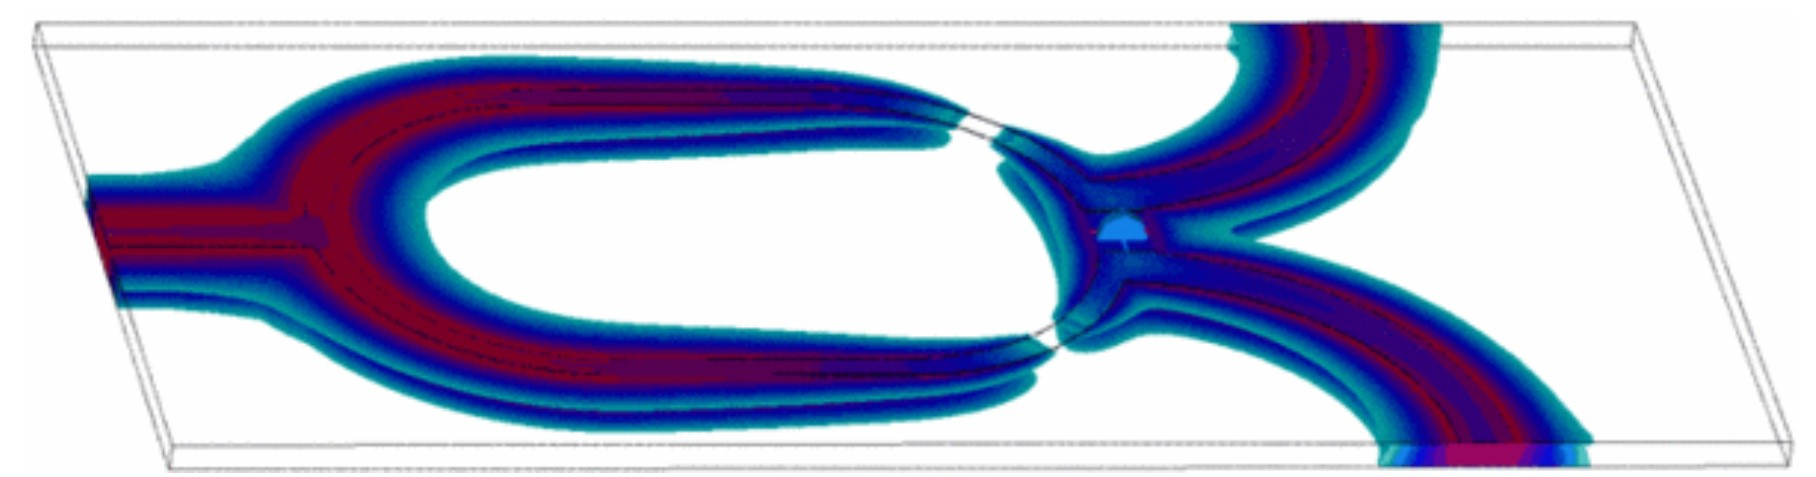
\includegraphics[width=8cm]{imagenes/img2}
        \caption{E-field phase animation of a Wilkinson power dividerpozar2012microwave.}
        \label{fig:animation}
\end{figure}
\section{Problema}
\label{sec:Problem}
La division de una señal de entrada en señales de salida equiamplitud y equifase se logra con un divisor tipo T o un divisor resistivo,pero estos presentan la limitacion de tan solo poseer un numero par de salidas, por ejemplo en caso se necesitaran usar 9 salidas, un divisor de 16 salidas tendria que ser utlizado, esto produciria disipación de potencia innecesaria,el divisor de potencia de Wilkinson soluciona este problema \cite{wilkinson1960n}.
\section{Fundamento Teórico}
\label{sec:fundamento}
Los divisores de potencia son caracterizados por matrices de dispersión que nos diran cual sera el comportamiento de dicho divisor, esta matriz es cuadrada cuyo orden dependerá del numero de puertos utilizados en nuestro caso sera de orden 3, ademas de ello si se analizan sus propiedades podremos saber si esta pertenece a un acoplador, divisivor de potencia y las carateristicas de los puertos de estas\cite{pozar2012microwave}. El divisor de potencia de Wilkinson es un dispositivo en el que todos los puertos estan emparejados,auque sea un dispositivo de N puertos normalmente lo encontramos como un divisor de 2 vias(3 puertos),no tiene perdidas cuando se excita el puerto de entrada y los puertos de salida se mantienen aislados.
\vspace{5mm}
\begin{equation}
[S]=
\begin{pmatrix}
S_{11}&S_{12}&S_{13}\\
S_{21}&S_{22}&S_{23}\\
S_{31}&S_{32}&S_{33}\\
\end{pmatrix}
\label{eq:scattering}
\end{equation}
Scattering matrix \ref{eq:scattering}.
\vspace{5mm}

Para analizar totalmente esta estructura realizaremos un análisis de modo par-impar, para dicho análisis partiremos el divisor de potencia como se muestra en la figura \ref{fig:Analisis}.
\vspace{50mm}
\begin{figure}[h]
    \centering
        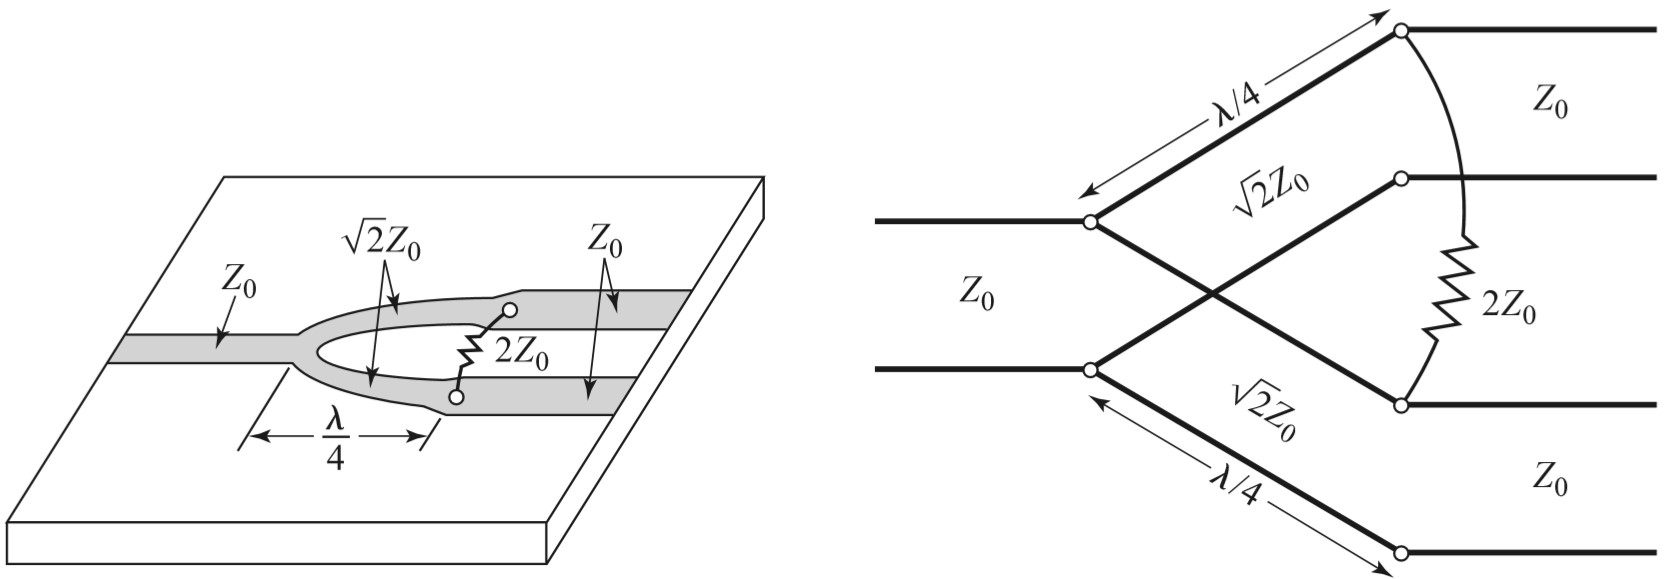
\includegraphics[width=8cm]{imagenes/img17}
        \caption{Division del divisor de potencia de Wilkinson}
        \label{fig:Analisis}
\end{figure}
\begin{figure}[h]
    \centering
    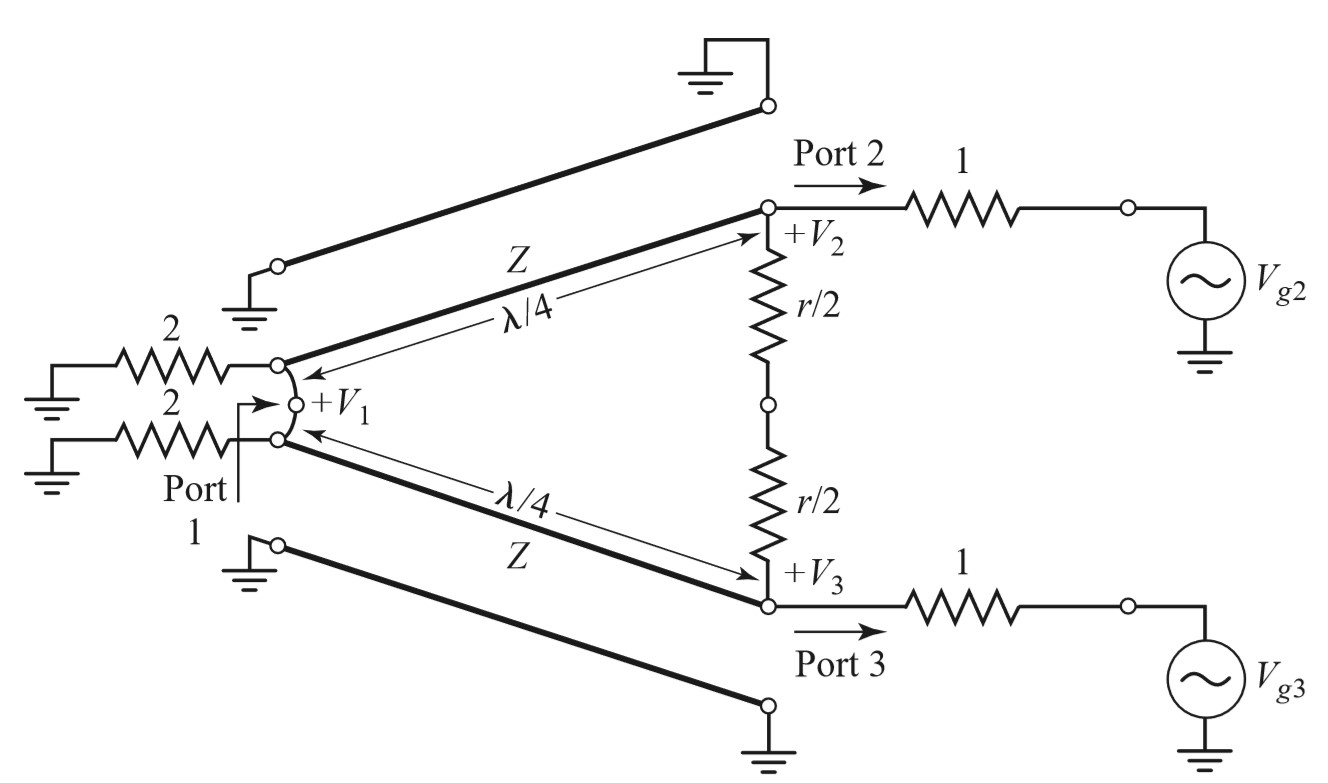
\includegraphics[width=8cm]{imagenes/img3}
    \caption{Diagrama Esquematico del divisor de potencia de Wilkinson.}
    \label{fig:diagrama}
\end{figure}
\begin{figure}[h]    
    \centering
        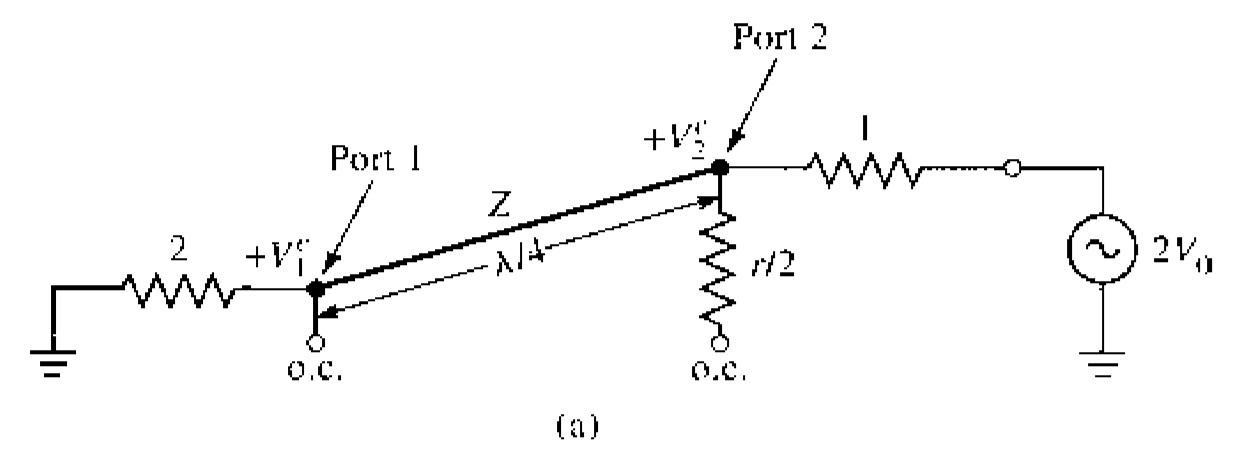
\includegraphics[width=8cm]{imagenes/img4}
        \caption{Analisis Par-Impar.}
        \label{fig:analisis-par-impar}
\end{figure}
Posteriormente como resultado de este análisis tendremos los siguientes parametros de dispersion. 
\begin{equation}
\begin{split}
    S_{11}&=0 \\
    S_{22}&=S_{33}=0 \\
    S_{12}&=S_{21}=-\frac{j}{\sqrt{2}}\\
    S_{13}&=S_{31}=-\frac{j}{\sqrt{2}}\\
    S_{23}&=S_{32}=0
\end{split}
    \label{eq:parametros}
\end{equation}
La matriz de dispersión del modelo que se simulará es la siguiente
\begin{equation}
    \begin{pmatrix}
    0&-\frac{j}{\sqrt{2}}&-\frac{j}{\sqrt{2}}\\
    -\frac{j}{\sqrt{2}}&0&0\\
    -\frac{j}{\sqrt{2}}&0&0\\
    \end{pmatrix}
    \label{eq:matrix_numbers}
\end{equation}
\section{El modelo}
Se utilizará CST Studio Suite para el modelamiento de este divisor, los parametros a utilizar en la simulación estan dados en el cuadro \ref{tab:parametros_simulacion} \cite{cstpage}.
\begin{table}[h]
    \caption{Tabla de Parametros}
\begin{tabular}{@{}lll@{}}
\toprule
Parametro & Valor    & Descripción \\ \midrule
h         & 1.2 mm   & Grosor del Substrato \\
eps\_r    & 4.3      & Permitividad del Substrato \\
t         & 0.035 mm & Espesor de metalización \\ 
W50       & 2.35 mm  & 50 Ohms (Z0) Anchura de linea \\
W70       & 1.23 mm  & 70.71 Omhs (Z0$\sqrt{2}$) \\
l70       & 42.54 mm & Longitud de Lambda / 4 del ancho de línea Z0$\sqrt{2}$\\ \bottomrule
\end{tabular}
\label{tab:parametros_simulacion}
\end{table}

Procederemos a abrir CST Studio Suite, usaremos la plantilla de Planar Coupler and Divider, en modo time domain solver y configuraremos los monitores de campo eléctrico, magnético y flujo de potencia, que usaremos para visualizar los resultados de la simulación.
Seguidamente ingresaremos los parametros de la tabla \ref{tab:parametros_simulacion} como se muestra en la figura.

\begin{figure}[h]    
    \centering
        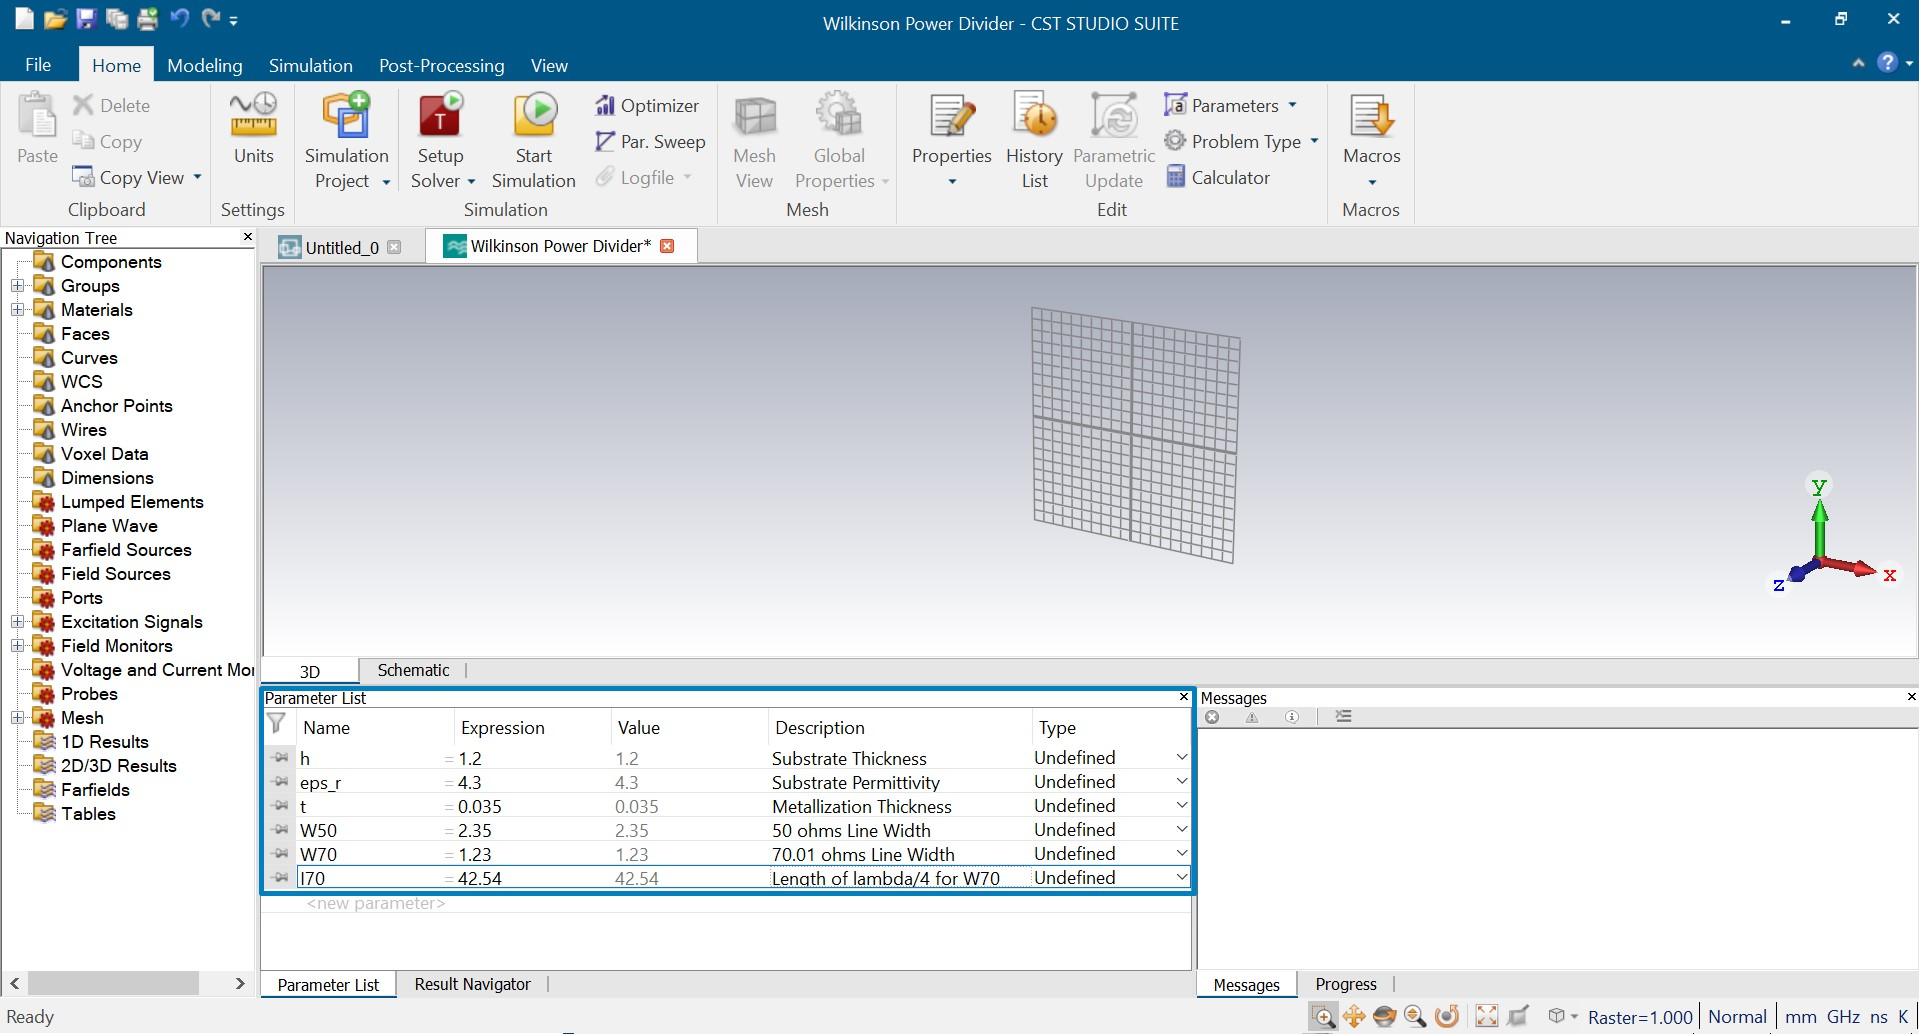
\includegraphics[width=9cm]{imagenes/img5}
        \caption{Ingreso de Parametros de Simulación.}
        \label{fig:ingreso_de_parametros}
\end{figure} 
Una vez los parametros esten ingresados podremos usar sus valores usando sus nombres en cualquier momento de la simulación.

Usaremos los parametros para empezar a construir el divisor de potencia, utilizaremos las herramientas para modelado 3D y las transformaciones disponibles para lograr la geeometria deseada, se muestran imagenes de este proceso.

\begin{figure}[h]    
    \centering
        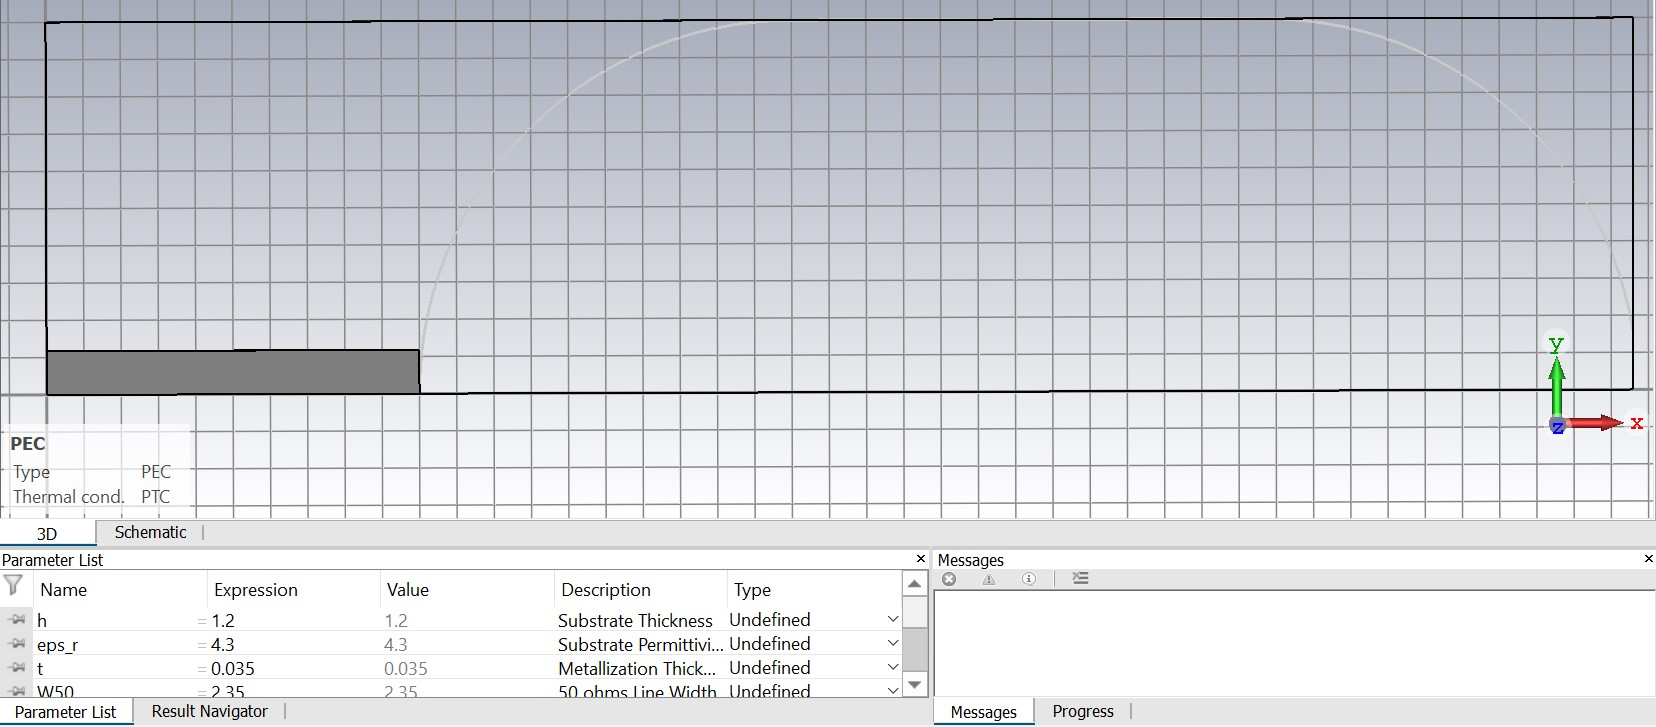
\includegraphics[width=9cm]{imagenes/img6}
        \caption{Ingreso de Parametros de Simulación.}
        \label{fig:modelamiento1}
\end{figure} 
\vspace{50mm}
\begin{figure}[h]    
    \centering
        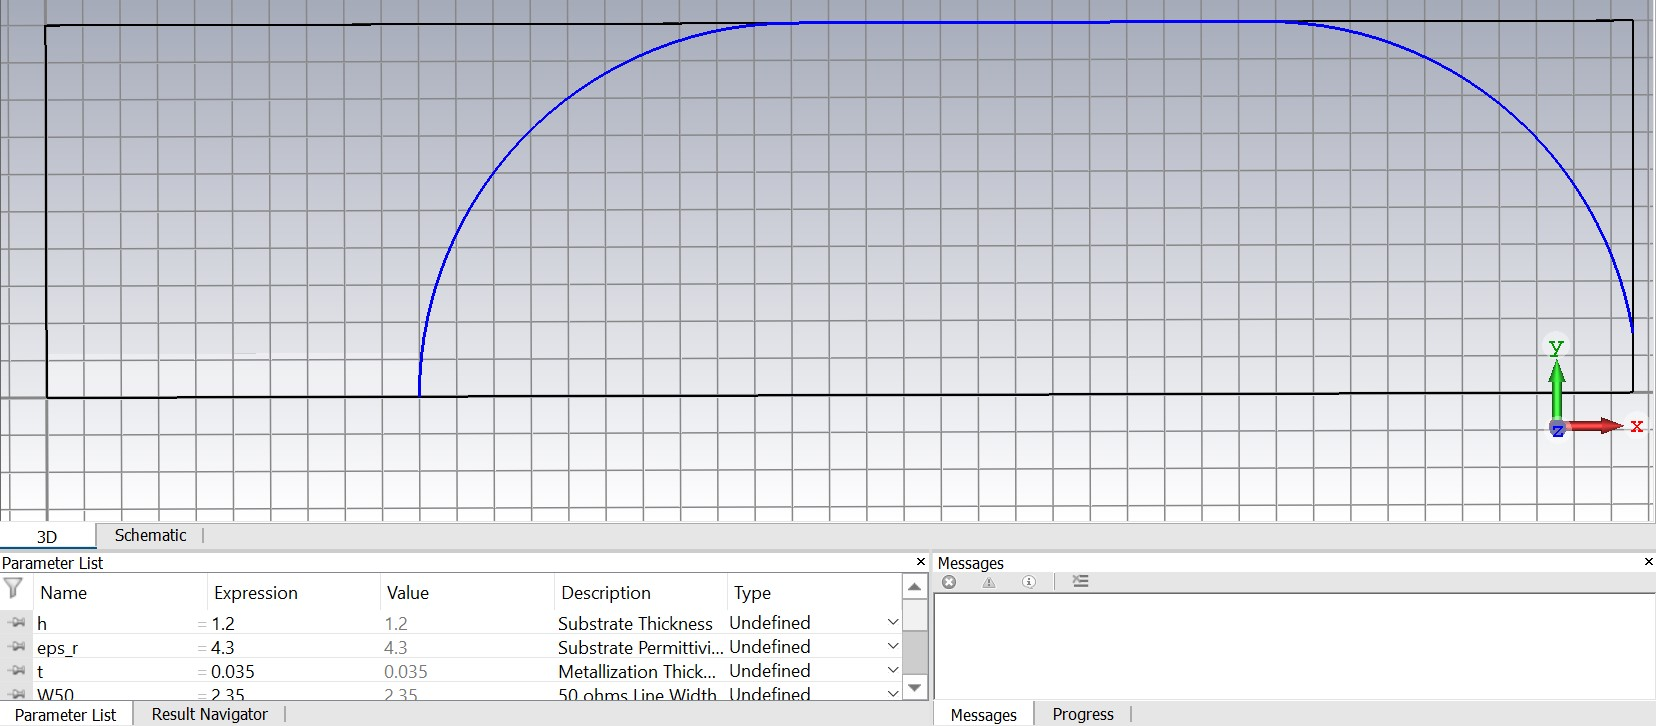
\includegraphics[width=9cm]{imagenes/img7}
        \caption{Ingreso de Parametros de Simulación.}
        \label{fig:modelamiento2}
\end{figure} 
\begin{figure}[h]    
    \centering
        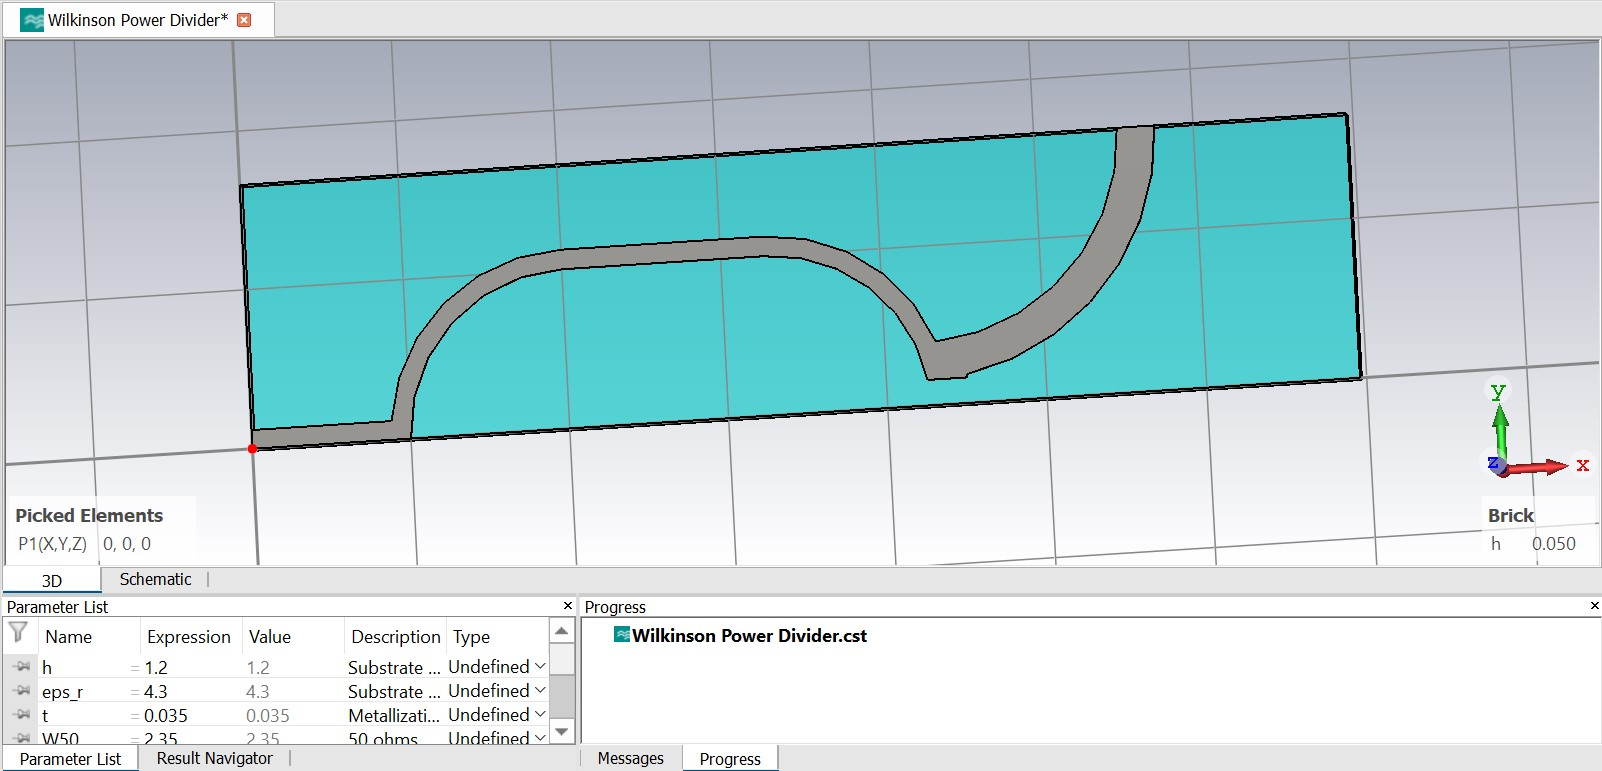
\includegraphics[width=9cm]{imagenes/img8}
        \caption{Ingreso de Parametros de Simulación.}
        \label{fig:modelamiento3}
\end{figure} 

Se aprovechará la simetria del modelo para su construcción, gracias a esto, solo será necesario construir una mitad del divisor y aplicar la transformación del espejo para construir la otra mitad. La línea de entrada es de 50 Omhs. 
\begin{figure}[h]    
    \centering
    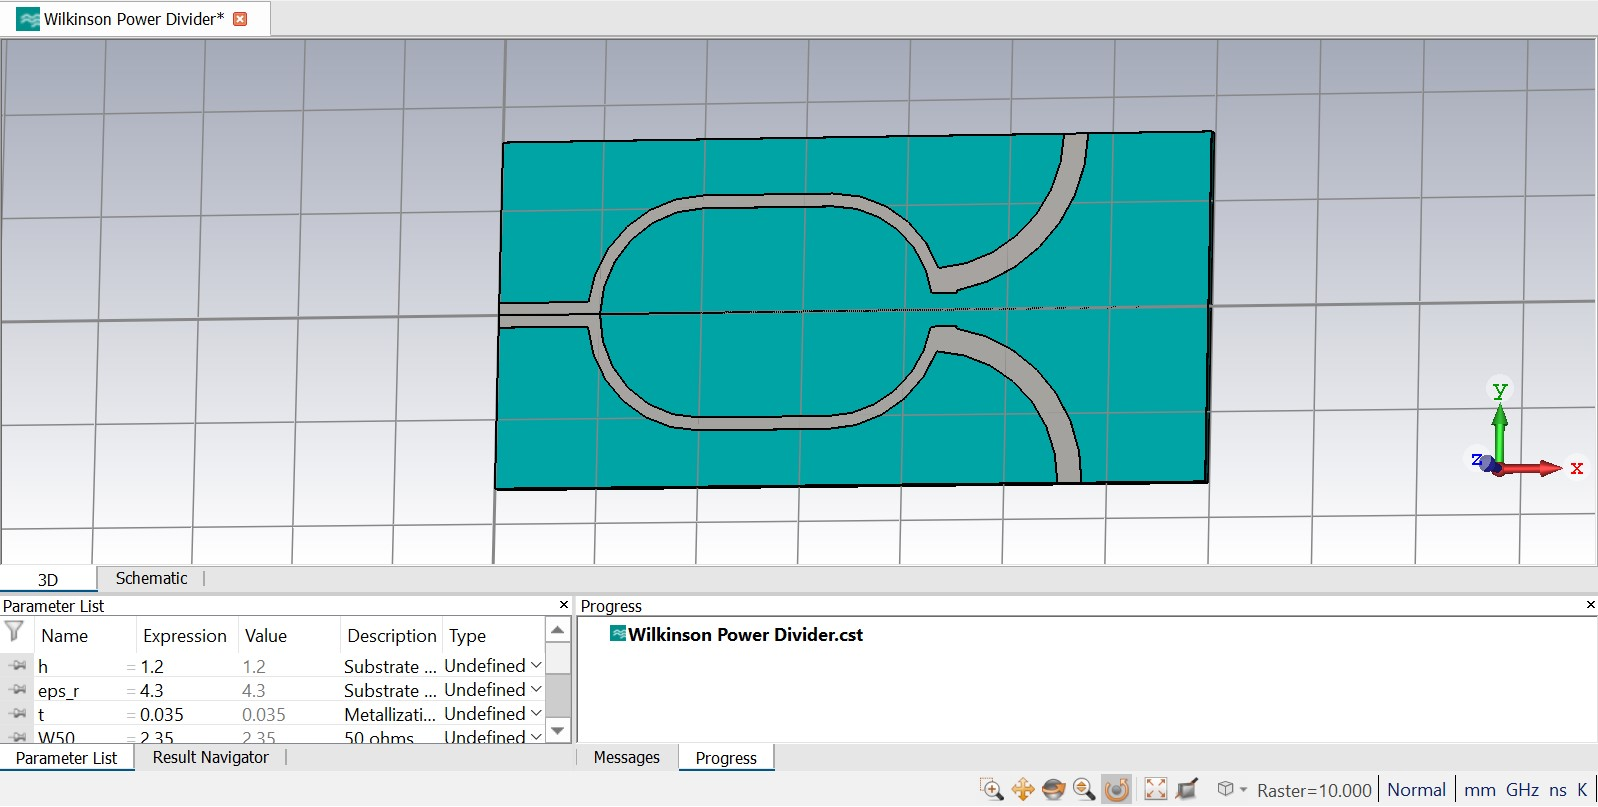
\includegraphics[width=9cm]{imagenes/img9}
    \caption{Ingreso de Parametros de Simulación.}
    \label{fig:modelamiento4}
\end{figure} 
%\vspace{15mm}

Se incluirá una resistencia SMD de 100 Ohms entre las ramas del divisor, esto se muestra en la figura \ref{fig:modelamiento5}.
\begin{figure}[h]    
    \centering
    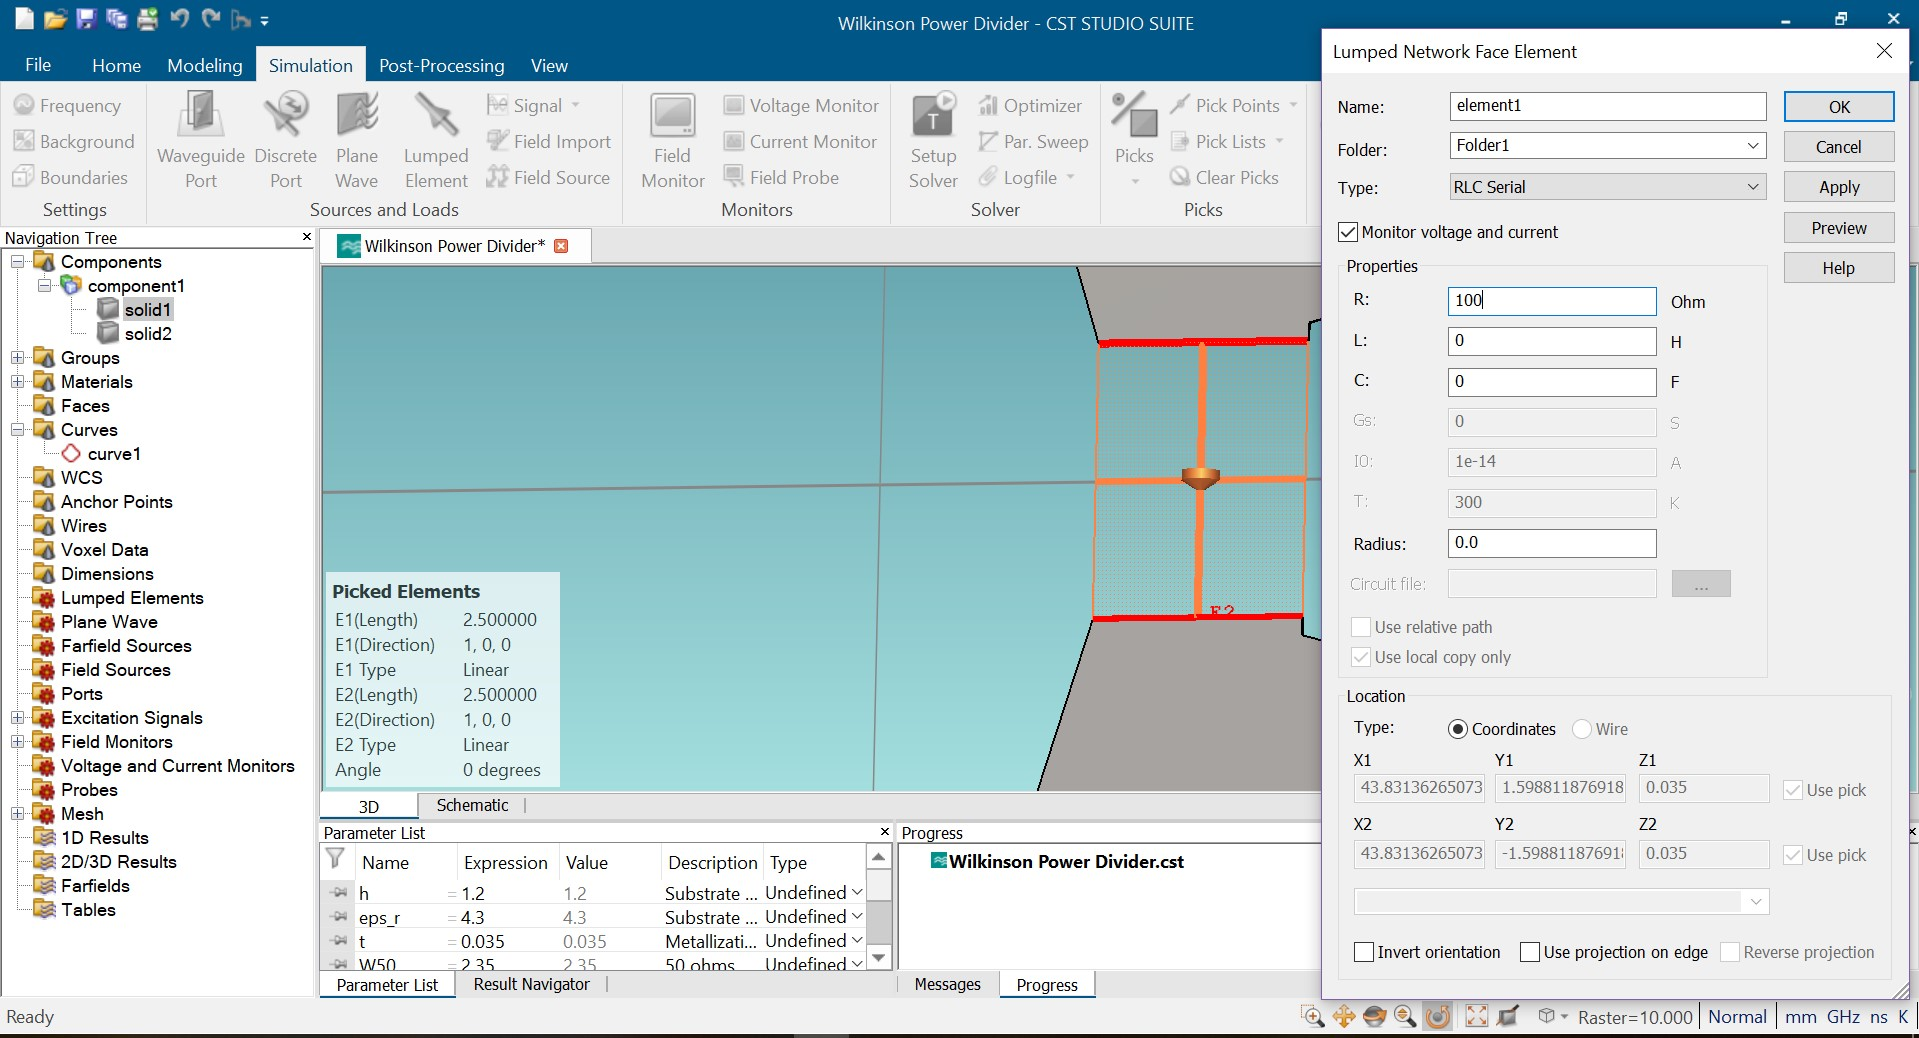
\includegraphics[width=9cm,height=3.403cm]{imagenes/img10}
    \caption{Ingreso de Parametros de Simulación.}
    \label{fig:modelamiento5}
\end{figure} 
%\vspace{25mm}

Se configurarán los puertos del divisor, esto se muestra en la figura \ref{fig:modelamiento6}.
\begin{figure}[h]    
    \centering
    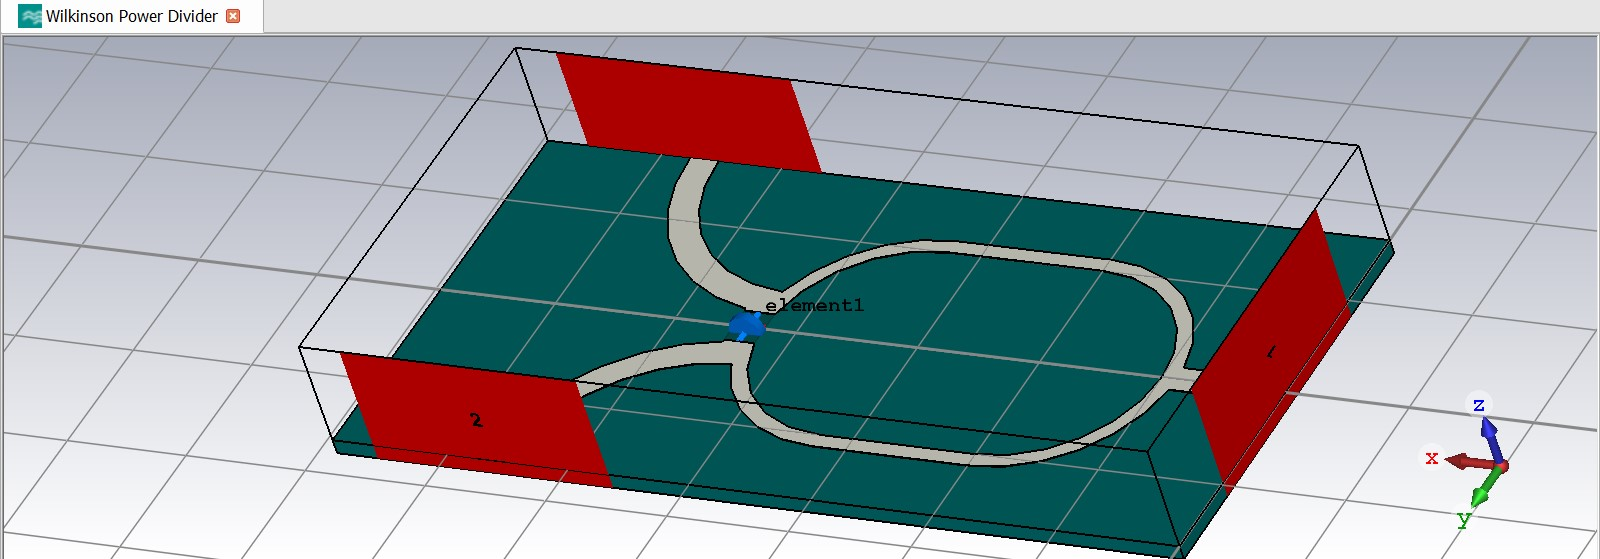
\includegraphics[width=9cm]{imagenes/img11}
    \caption{Ingreso de Parametros de Simulación.}
    \label{fig:modelamiento6}
\end{figure}
%\vspace{25mm}

Finalmente configuraremos los parametros del solver en el dominio del tiempo para ejecutar la simulación.
\begin{figure}[h]    
    \centering
    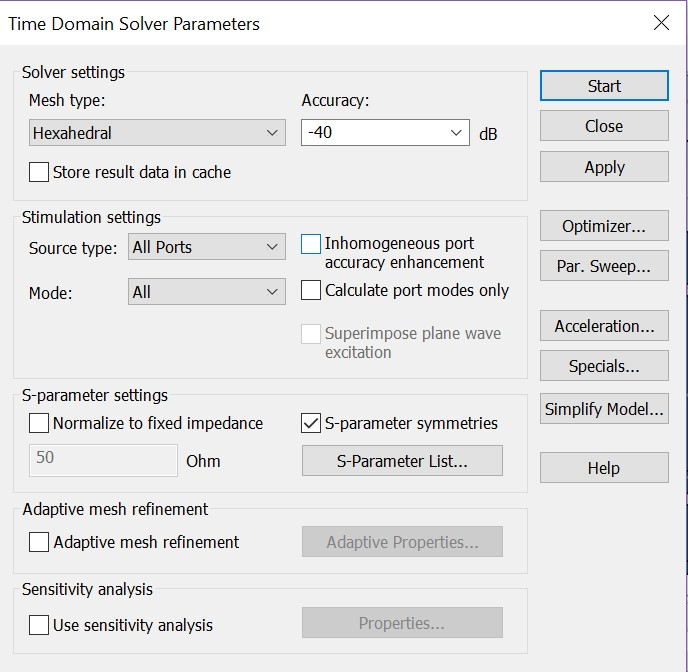
\includegraphics[width=9cm]{imagenes/img12}
    \caption{Ingreso de Parametros de Simulación.}
    \label{fig:modelamiento7}
\end{figure}

Podremos visualizar el campo eléctrico y el campo magnético en el divisor para distintas fases pudiendo incluso mostrar una animacion de esta variando, asi como una variedad de gráficos que proporcionan información relevante acerca del divisor.

\begin{figure}[h]    
    \centering
    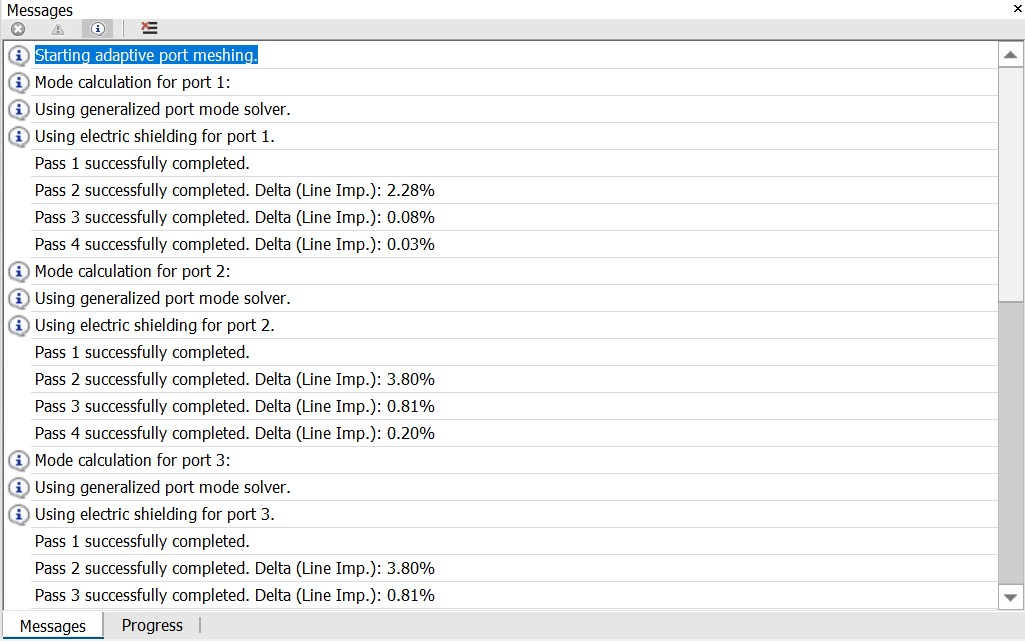
\includegraphics[width=9cm,height=4.4cm]{imagenes/img13}
    \caption{Ingreso de Parametros de Simulación.}
    \label{fig:modelamiento8}
\end{figure}
\vspace{10mm}
\begin{figure}[h]    
    \centering
    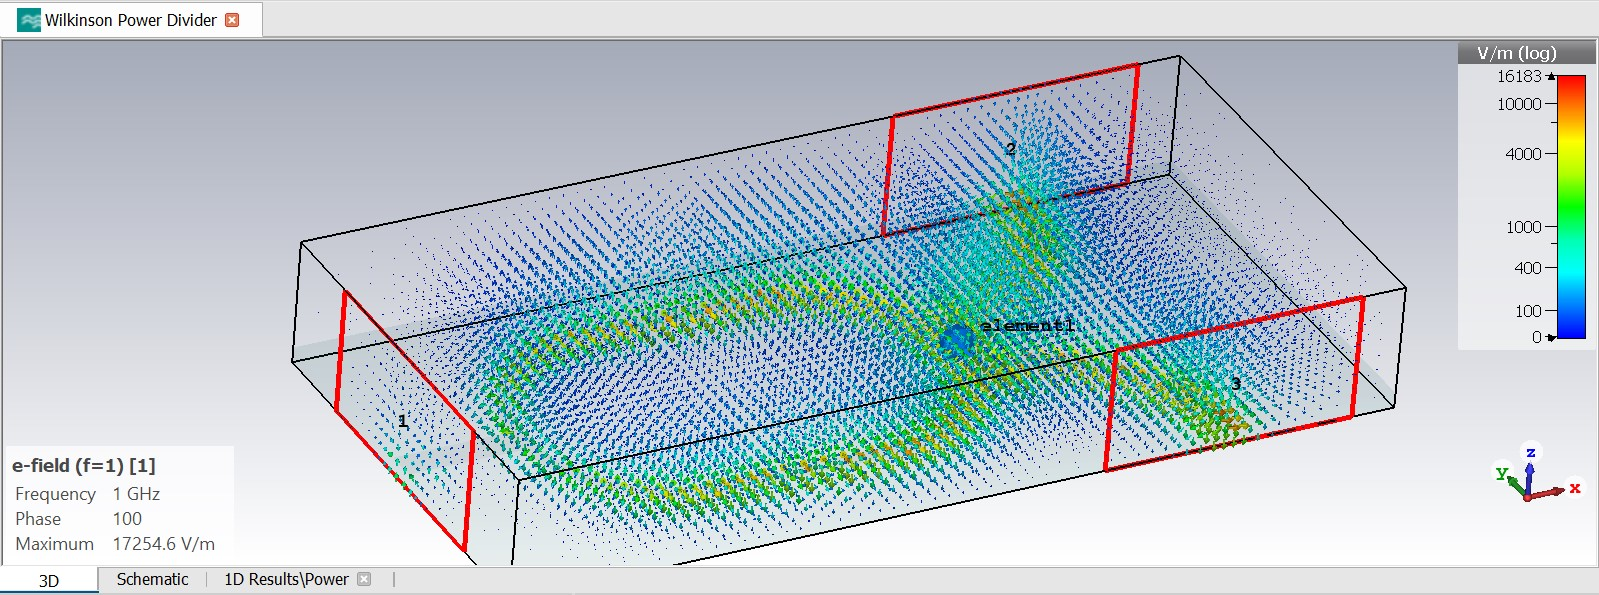
\includegraphics[width=9cm]{imagenes/img15}
    \caption{Ingreso de Parametros de Simulación.}
    \label{fig:modelamiento9}
\end{figure}
\begin{figure}[h]    
    \centering
    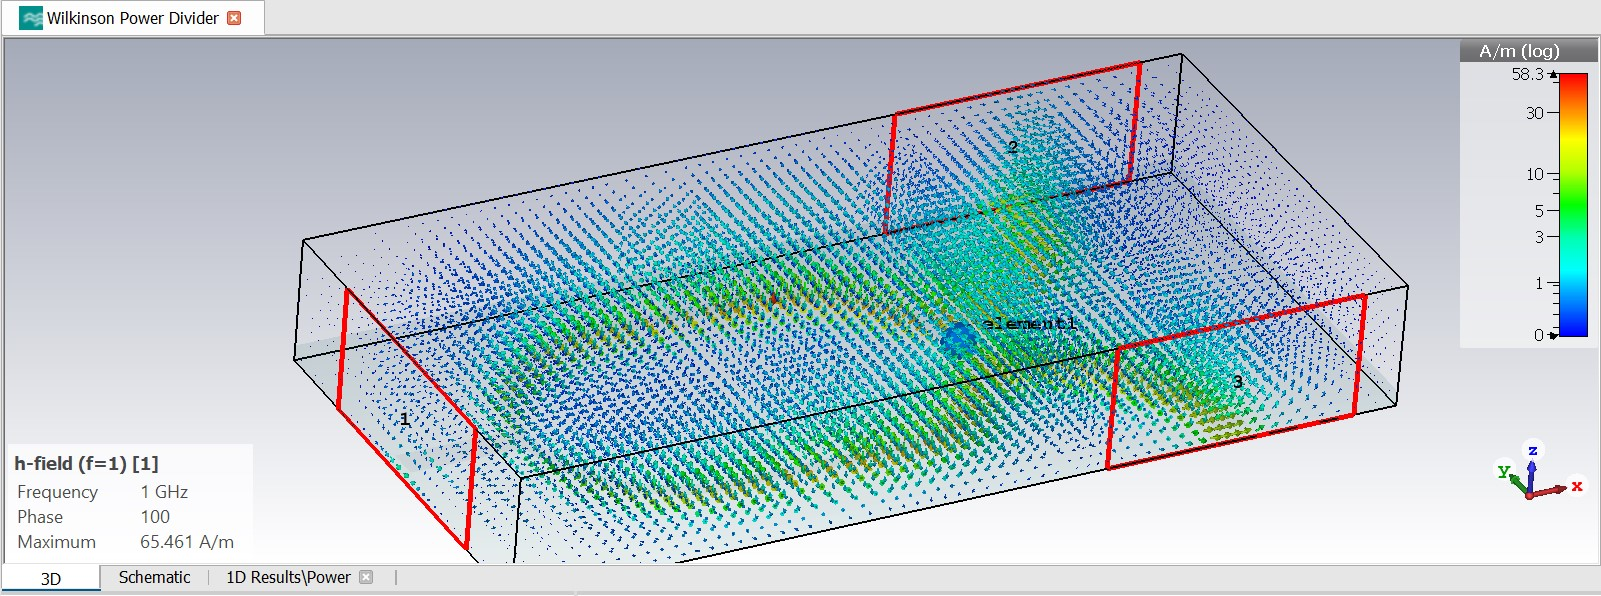
\includegraphics[width=9cm]{imagenes/img16}
    \caption{Ingreso de Parametros de Simulación.}
    \label{fig:modelamiento10}
\end{figure}

%\vspace{10mm}
Bibliografía
\bibliographystyle{ieeetr}
\bibliography{bibliografia}
\end{document}